% folded pyramid P-ACFE with AB base, PE vertical, F on BC, D foot on AB
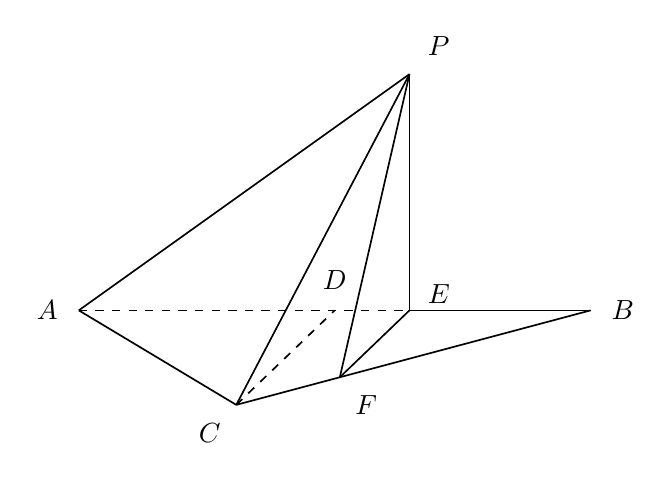
\begin{tikzpicture}[x=1cm,y=1cm,line width=0.6pt,font=\normalsize]
\coordinate (A) at (0,1.2);
\coordinate (B) at (6.5,1.2);
\coordinate (E) at (4.2,1.2);
\coordinate (D) at (3.2500000000,1.2000000000);
\coordinate (C) at (2.0,0);
\coordinate (F) at (3.3153846154,0.3507692308);
\coordinate (P) at (4.2,4.2);
% base AB: A-E dashed (with D on it), E-B solid
\draw[dashed] (A) -- (E);
\draw (E) -- (B);
% base BC with F on it solid
\draw (C) -- (B);
% base AC solid
\draw (A) -- (C);
% vertical and slant edges solid
\draw (P) -- (A);
\draw (P) -- (E);
\draw (P) -- (C);
\draw (P) -- (F);
\draw (E) -- (F);
% hidden altitude CD dashed
\draw[dashed] (C) -- (D);
% labels offset to avoid strokes
\node[left,xshift=-4pt,yshift=0pt] at (A) {$A$};
\node[right,xshift=4pt,yshift=0pt] at (B) {$B$};
\node[right,xshift=3pt,yshift=6pt] at (E) {$E$};
\node[above,xshift=0pt,yshift=4pt] at (D) {$D$};
\node[below left,xshift=-2pt,yshift=-3pt] at (C) {$C$};
\node[below right,xshift=2pt,yshift=-3pt] at (F) {$F$};
\node[above right,xshift=3pt,yshift=3pt] at (P) {$P$};
\end{tikzpicture}
